\documentclass[a4paper,12pt]{article} %style de document
\usepackage[utf8]{inputenc} %encodage des caractères
\usepackage[french]{babel} %paquet de langue français
\usepackage[T1]{fontenc} %encodage de la police
\usepackage[top=2cm,bottom=2cm,left=2cm,right=2cm]{geometry} %marges
\usepackage{graphicx} %affichage des images


\begin{document} %début du document



%----------------------------------
%page de garde
%----------------------------------

\begin{titlepage}

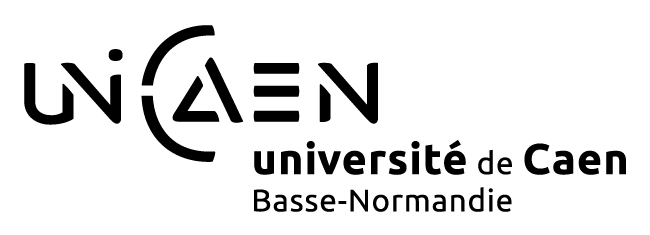
\includegraphics[scale=0.3]{images/unicaen.png}

\vspace{7cm}

\begin{center}

\begin{Huge}
Complément POO\\
Rapport du Devoir\\
\end{Huge}
\vspace{2cm}
\begin{large}
Beauchamp Aymeric 21301016\\
Chagneux Dimitri 21606807\\
Mori Baptiste 21602052\\
Leblond Valentin 21609038\\
\vspace{1cm}
L2-Info-groupe-4A
\end{large}

\end{center}
\end{titlepage}


%------------------------------
%sommaire
%------------------------------

\newpage

\tableofcontents{}

\newpage

%------------------------------
%contenu
%------------------------------


\section*{Introduction}
\addcontentsline{toc}{section}{Introduction}

L'objectif de ce projet étant de réaliser un Taquin qui est un casse-tête consistant à déplacer des cases d'un plateau afin de les replacer dans l'ordre et de reconstituer l'image ou le paterne souhaité.

\begin{figure}[!h]
\centering
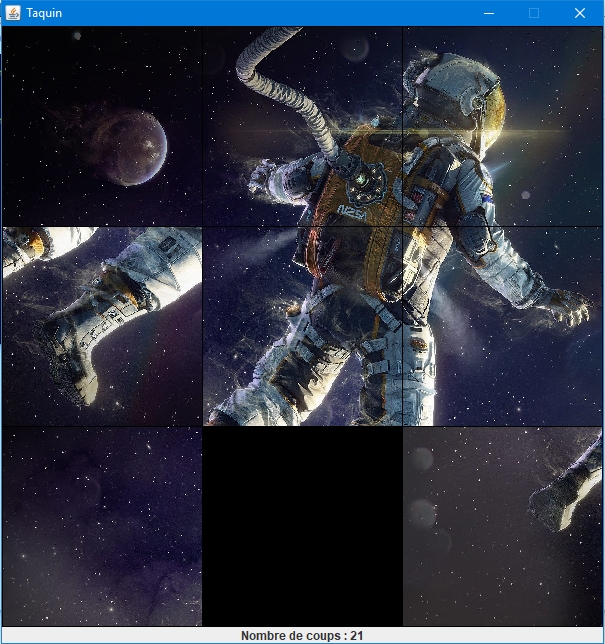
\includegraphics[scale=0.5]{images/Capture.PNG}
\caption{Jeu du Taquin}
\end{figure}

Nous avons séparé le projet en deux packages, le premier comporte la version console avec la structure du jeu (le package \textbf{model}) et le deuxième contient toute la partie graphique (le package \textbf{GUI}), nous avons un troisième dossier qui possède les images pour l'interface graphique (le package \textbf{ressources}).

\section{La conception du package model}

\subsection{Organisation des classes}

Tout d'abord, nous avons représenté les cases par deux types de classe, FullTile pour les cases pleines et EmptyTile pour la zone vide qu'on déplacera. Ces deux classes possède des attributs en commun qui sont les coordonnées X et Y de la case c'est pourquoi on a fait une classe abstraite Tile qui possède ces coordonnées.\\
La classe FullTile possède un identifiant sous forme d'entier qui la caractérise des autres cases, on s'arrangera donc à leur mettre une valeur différente pour chaqu'une de ces cases.\\

Ensuite, nous avons une classe Board qui représentera l'état du jeux et qui fera en sorte de déplacer la case vide, résoudre le niveau avec un solveur, mélanger le jeu, etc.

\begin{figure}[!h]
\centering
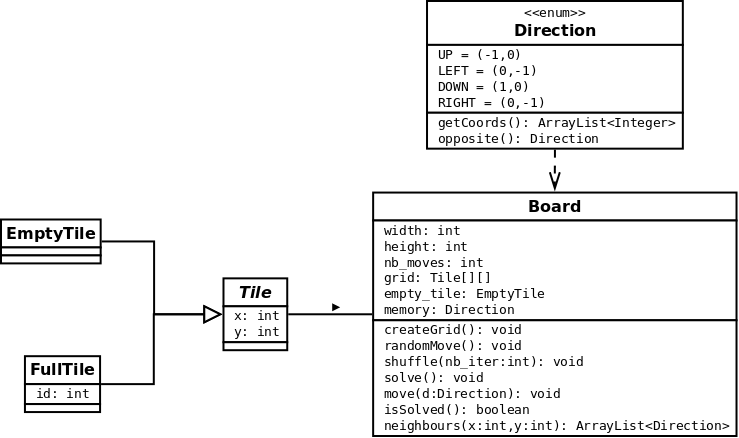
\includegraphics[scale=0.4]{images/model.png}
\caption{Diagramme de classe du package model}
\end{figure}

\newpage

\subsection{Algorithmes du Board}

Tout d'abord, nous avons une fonction \textbf{createGrid} qui permet d'initialiser une grille avec des FullTile et une EmptyTile et une fonction \textbf{toString} qui permet de l'afficher.

\begin{figure}[!h]
\centering
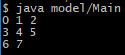
\includegraphics[scale=1]{images/Capture2.PNG}
\caption{Affiche d'une grille 3x3 initialisée}
\end{figure}

Ensuite, nous avons créer les déplacements de la case vide, nous avons d'abord commencer par créer des énums UP, DOWN, LEFT, RIGHT qui représentent à la direction de déplacement de la case vide.


\end{document}
